\documentclass[
superscriptaddress,
amsmath,
amssymb,
aps,
prl,
twocolumn,
floatfix
]{revtex4-1}
\usepackage{graphicx}          % Include figure files
\usepackage{dcolumn}           % Align table columns on decimal point
\usepackage{bm}                % bold math
\usepackage{units}             % set units in a typographically correct way
\usepackage[usenames,dvipsnames]{color}
\usepackage[colorlinks,urlcolor=blue,citecolor=blue,linkcolor=blue]{hyperref}
\usepackage{upgreek}
\usepackage[T1]{fontenc}
\usepackage[utf8]{inputenc}

% MACROS
% AMO abbreviations
\def\kr{k_{\rm R}}                                    % kr
\def\Er{E_{\rm R}}                                    % kr
\def\Rb87{^{87}\mathrm{Rb}}                     % Rb 87
\def\K40{^{40}\mathrm{K}}                       % K 40

% Unit vectors
\def\ex{\mathbf{e}_x}
\def\ey{\mathbf{e}_y}
\def\ez{\mathbf{e}_z}

%bra/ket commands
\def\bra#1{\mathinner{\langle{#1}|}}
\def\ket#1{\mathinner{|{#1}\rangle}}
\def\braket#1{\mathinner{\langle{#1}\rangle}}
\def\Bra#1{\left<#1\right|}
\def\Ket#1{\left|#1\right>}
{\catcode`\|=\active
  \gdef\Braket#1{\left<\mathcode`\|"8000\let|\BraVert {#1}\right>}}
\def\BraVert{\egroup\,\mid@vertical\,\bgroup}

% Editorial macros
\newcommand{\reffig}[1]{\mbox{Fig.~\ref{#1}}}
\newcommand{\refeq}[1]{\mbox{Eq.~(\ref{#1})}}
\newcommand{\refsec}[1]{\mbox{Sec.~(\ref{#1})}}
\newcommand{\etal}{et~al.}
\newcommand{\note}[1]{\textcolor{ForestGreen}{[\textrm{#1}]}} % Make editorial notes green
% \newcommand{\note}[1]{\textcolor{ForestGreen}{[]}} % Empty editorial notes

\def\shorttimes{\!\times\!}

\addtolength{\abovecaptionskip}{-0.1in}
\addtolength{\belowcaptionskip}{-0.2in}

%
% Enable/disable supporting computations
%
\usepackage{etoolbox}
\newtoggle{SUPPORT}
\toggletrue{SUPPORT}
%\togglefalse{SUPPORT}
\long\def\support#1{ \iftoggle{SUPPORT}{\begin{widetext}\small {\leavevmode\color{red}{#1}} \normalsize\end{widetext}}{} }


\begin{document}

\title{Magnetic field stabilization in ultracold atom experiments using partial transfer absorption imaging}

% \author{R. P. Anderson}
% \thanks{These two authors contributed equally.}
% \affiliation{Joint Quantum Institute, University of Maryland, College Park, Maryland, 20742, USA}
% \affiliation{School of Physics and Astronomy, Monash University, Melbourne, Victoria 3800, Australia}
% \affiliation{La Trobe Institute of Molecular Science, La Trobe University, Bendigo, Victoria 3552, Australia}

% \author{D. Trypogeorgos}
% \thanks{These two authors contributed equally.}
% \affiliation{INO-CNR BEC Center and Dipartimento di Fisica, Universit\`a di Trento, 38123 Povo, Italy}
% \affiliation{Joint Quantum Institute, University of Maryland, College Park, Maryland, 20742, USA}

\author{A. Vald\'es-Curiel}
\author{Q.-Y. Liang}
\author{J. Tao}
\author{M. Zhao}
\affiliation{Joint Quantum Institute, University of Maryland, College Park, Maryland, 20742, USA}

\author{I. B. Spielman}
\email{ian.spielman@nist.gov}
\homepage{http://ultracold.jqi.umd.edu}
\affiliation{Joint Quantum Institute, University of Maryland, College Park, Maryland, 20742, USA}
\affiliation{National Institute of Standards and Technology, Gaithersburg, Maryland 20899, USA}

\date{\today}%

\begin{abstract}
We present a non-destructive method for measuring and stabilizing magnetic fields in ultracold atom experiments using partial transfer absorption imaging. 
\end{abstract}

\maketitle

%%%%%%%%%%%%%%%%%%%%%%%%%%%%%%%%%%%%%%%%%%%%%%%%%%%%%%%%%%%%%%%%%%
%
% Introduction and context
%
%%%%%%%%%%%%%%%%%%%%%%%%%%%%%%%%%%%%%%%%%%%%%%%%%%%%%%%%%%%%%%%%%%

This is the introduction

%%%%%%%%%%%%%%%%%%%%%%%%%%%%%%%%%%%%%%%%%%%%%%%%%%%%%%%%%%%%%%%%%%
%
% Proposal
%
%%%%%%%%%%%%%%%%%%%%%%%%%%%%%%%%%%%%%%%%%%%%%%%%%%%%%%%%%%%%%%%%%%

{\it Proposal} 

The population transfered by the microwave pulse is 

\begin{equation}
	P_e(\Omega, \delta, t)=\frac{\Omega^2}{\Omega^2+\delta^2}\sin^2\left(\frac{\sqrt{\Omega^2+\delta^2}}{2}t\right)
	\label{eq:Rabi_oscillations}	
\end{equation}

The full width half maximum is $1/t$. Set $\Omega$ and $t$ such that $P_e<0.05$

Each pulse 
\begin{equation}
	n_\pm = n_0 P_e(\Omega, \delta_+, \tau)
\end{equation}

with $\delta_+=\delta_0+1/(2\tau)$ 

Second pulse:
\begin{equation}
	n_-=(n_0-n_+)P_e(\Omega, \delta_-, \tau)\approx n_0P_e(\Omega, \delta_-, \tau)
\end{equation}

The transfer function is 
\begin{equation}
	g(\Omega, \delta_0, \tau)
\end{equation}


Main contributions are shot noise and technical noise of the detector. 
{\it Signal to noise ratio}
SNR for absorption imaging according to Erin's paper is 
\begin{equation}
	SNR_{\mathrm{model}}=\frac{OD}{\Delta_0}\left(\frac{2}{1+e^{OD}}\right)^{1/2}
\end{equation}

where $\Delta_0$ is the noise in the absence of atoms.

Write transfer function, propagate uncertainties in n transferred to get the real transfer function. 



{\it Dick effect}

Dick effect due to non-continuous probing 


%%%%%%%%%%%%%%%%%%%%%%%%%%%%%%%%%%%%%%%%%%%%%%%%%%%%%%%%%%%%%%%%%%
%
% Basic experimental details 
%
%%%%%%%%%%%%%%%%%%%%%%%%%%%%%%%%%%%%%%%%%%%%%%%%%%%%%%%%%%%%%%%%%%

{\it Implementation} 

Most experiments are performed in the $F=1$ ground hyperfine manifold with some bias field $B_0\ez$ that shifts the energies of the different $\ket{m_F}$ states. Due to the linear dependence of the energies of the $\ket{m_F=\pm1}$ and the constant changes in the ambient magnetic field we use microwave assisted partial transfer absorption imaging (PTAI) to monitor and stabilize the magnetic field. 

The method relies on transferring a small fraction of atoms into the $5^2S_{1/2}$ $F=2$ manifold using an oscillating magnetic field with frequency close to the $\unit[6.8]{GHz}$ ground hyperfine splitting. The atoms in $F=2$ can be imaged without the use of repump light and therefore minimally disturbing the remaining atoms in $F=1$. We apply two microwave pulses for a total time $\tau$ with frequency $\omega_0-\delta_{\pm}$ where $\delta_{\pm}=\pm1/(2\tau)$. We typically set $\omega_0$ equal to the Zeeman splitting between the $\ket{F=1, m_f=-1}$ and $\ket{F=2, m_f=-2}$ states at a target magnetic field and we set the coupling strength $\Omega_0\ll 1/\tau$ such that only about $5\%$ of the atoms are transferred by each pulse. We image the transferred atoms following each pulse using absorption imaging and from the measured densities we calculate the imbalance or error
%
\begin{equation}
 	n_{\rm{imb}}=\frac{n(\delta_+)-n(\delta_-)}{n(\delta_+)+n(\delta_-)}
 \end{equation} 
%
\begin{figure}[htb]
\begin{center}
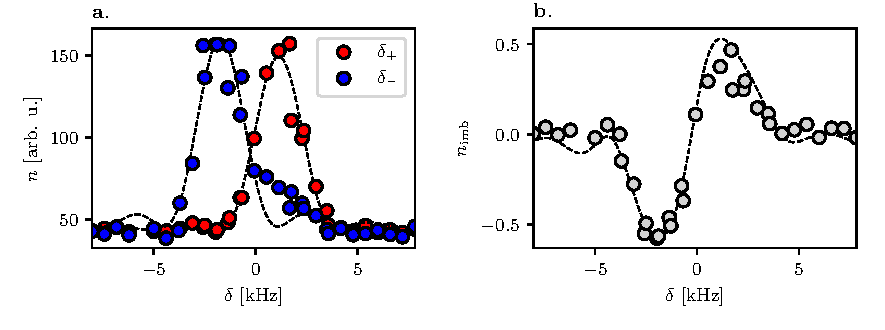
\includegraphics[]{Figures/uwave_lock.pdf}
\caption[Magnetic field stabilization using microwave assisted PTAI]{Magnetic field stabilization using microwave assisted PTAI. {\bf a.} Population transfered into $\ket{F=2, m_F=-1}$ from $\ket{F=1, m_F=-1}$ as a function of bias magnetic field (global detuning $\delta$). Each microwave pulse was $\tau=\unit[250]{\mu s}$ and detuned by $\delta_{\pm}=\pm 1/(2\tau)$ transfer a small fraction of atoms from $\ket{F=1, m_F=-1}$ into $\ket{F=2, m_F=-1}$. {\bf b.} Error signal calculated using the transfered atoms by each pulse. We lock the magnetic field to the $\sim\unit[5]{kHz}$ ($\unit[\sim 7]{mG}$) wide linear portion of the signal.}
\label{fig:uwave_lock}
\end{center}
\end{figure}
signal that is both insensitive to fluctuations in the number of atoms and linearly sensitive to changes in magnetic field\footnote{A single pulse on resonance is quadratically sensitive to detuning} . We use this error signal both to monitor the magnetic field before performing experiments and to cancel long term drifts in the field. In most cases, we chose the states $\ket{F=1, m_F=-1}$ and $\ket{F=2, mf=-2}$ as their relative energies are the most sensitive to changes in magnetic field. Figure~\ref{fig:uwave_lock}a shows the number of atoms transferred by each microwave pulse for different values of bias magnetic field and Figure~\ref{fig:uwave_lock}b shows the imbalance. The microwave frequency $\omega_0$ is on resonance with the $\ket{F=1, m_F=-1}\rightarrow\ket{F=2, m_F=-2}$ transition when both pulses transfer the same number of atoms.


In~\cite{seroka_repeated_2019} we studied partial transfer absorption imaging as a minimally destructive technique for imaging ultracold atoms.  
%%%%%%%%%%%%%%%%%%%%%%%%%%%%%%%%%%%%%%%%%%%%%%%%%%%%%%%%%%%%%%%%%%
%
% Results II: Resolution of BZ
%
%%%%%%%%%%%%%%%%%%%%%%%%%%%%%%%%%%%%%%%%%%%%%%%%%%%%%%%%%%%%%%%%%%

{\it Results}  

%%%%%%%%%%%%%%%%%%%%%%%%%%%%%%%%%%%%%%%%%%%%%%%%%%%%%%%%%%%%%%%%%%
%
% Results III: RF : 3x well lattice
%
%%%%%%%%%%%%%%%%%%%%%%%%%%%%%%%%%%%%%%%%%%%%%%%%%%%%%%%%%%%%%%%%%%


{\it More results maybe} 

%%%%%%%%%%%%%%%%%%%%%%%%%%%%%%%%%%%%%%%%%%%%%%%%%%%%%%%%%%%%%%%%%%
%
% Outlook
%
%%%%%%%%%%%%%%%%%%%%%%%%%%%%%%%%%%%%%%%%%%%%%%%%%%%%%%%%%%%%%%%%%%


\begin{acknowledgments}
This work was partially supported by the AFOSRs Quantum Matter MURI, NIST, and the NSF through the PFC at the JQI.
We are grateful for insights from the very detailed reading of our manuscript by G.~Reid and Y.~Yue.
\end{acknowledgments}

\bibliography{PTAI}

\end{document}

